%==================================================================%
% Author : Pando Muñoz, Manuel                                     %
%          Sánchez Barreiro, Pablo                                 %
% Version: 1.0, 30/03/2011                                         %
%                                                                  %
% Memoria del Proyecto Fin de Carrera                              %
% Archivo raíz para el capítulo de la arquitectura del sistema     %
%==================================================================%


\chapterheader{Arquitectura y diseño}{Definición Arquitectónica y Diseño Software}
\label{chap:arquitectura}

En el presente capítulo se presentan, mediante diagramas UML\cite{UML:2004, UML2:2004}, la arquitectura del sistema\cite{ARQ:2010}, los módulos de los que está compuesto, las comunicaciones existentes entre ellos, y el funcionamiento del mismo, es decir, se crea el marco de referencia que servirá de base para la construcción de la aplicación.

\chaptertoc

\section{Vista lógica de la arquitectura}
\label{sec:arquitectura:arqLogica}

En esta sección se describe la vista lógica de la arquitectura mediante un diagrama de componentes en la imagen \ref{fig:arquitectura:componentes}.
\newline


\begin{figure}
    \centering
    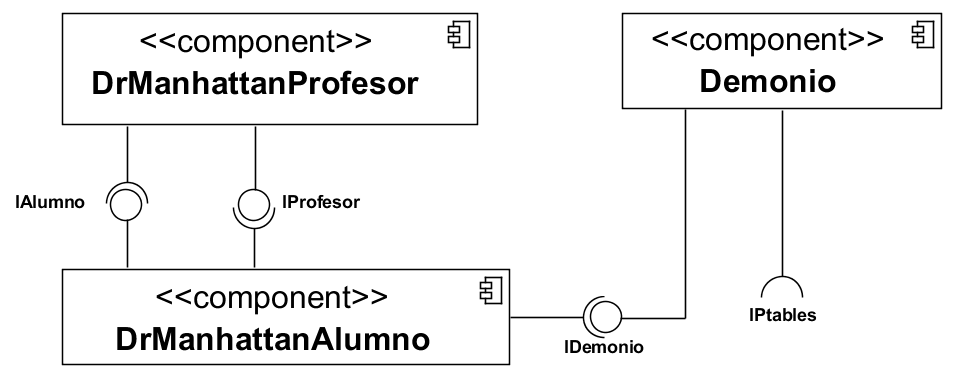
\includegraphics[width=\linewidth]{arquitectura/componentes}
    \caption{Diagrama de componentes}
    \label{fig:arquitectura:componentes}
\end{figure}


Los dos componentes principales \emph{DrManhattanProfesor} y \emph{DrManhattanAlumno} ofrecen cada uno interfaces de comunicación usadas por el otro. \emph{DrManhattanAlumno} también se comunica con una tercera parte del sistema, el \emph{Demonio}, que como vemos en la figura \ref{fig:arquitectura:despliegueSistema} forma parte de la aplicación del alumno. Este \emph{Demonio} es el encargado de comunicarse con \emph{iptables} cuándo hay que cambiar la política de acceso a la red.
\newline

\begin{figure}
    \centering
    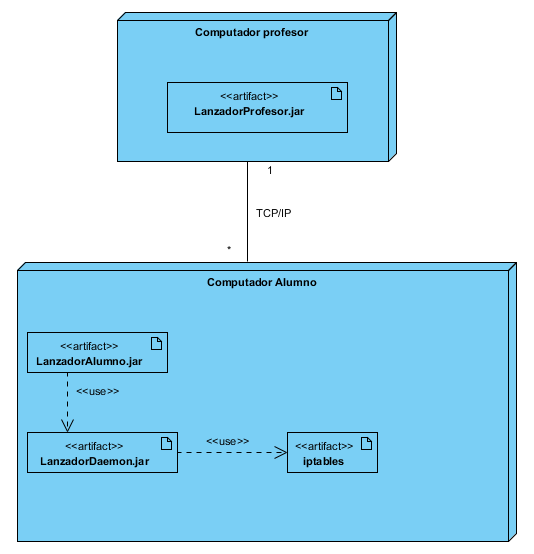
\includegraphics[width=\linewidth]{arquitectura/despliegueSistema}
    \caption{Diagrama despliegue del sistema}
    \label{fig:arquitectura:despliegueSistema}
\end{figure}

En la imagen \ref{fig:arquitectura:despliegueSistema} vemos la vista de despliegue del sistema. Tenemos dos tipos de computadores, en los que se ejecuta la aplicación del profesor, y en los que se ejecuta la del alumno.
\newline

Sólo se permite la existencia de una aplicación en el computador del profesor, a la que se conectan mediante TCP/IP un número indefinido de aplicaciones alumno, lógico, ya que en una prueba de una asignatura suelen ser varios los alumnos realizándola.
\newline


En la figura \ref{fig:arquitectura:actividadSistema} se muestran las posibles interacciones que tanto el alumno como el profesor realizan con sus respectivas aplicaciones durante el trascurso normal de una prueba, se siguen los pasos descritos en la sección \ref{sec:planificacion:descFuncional}.


\begin{figure}
    \centering
    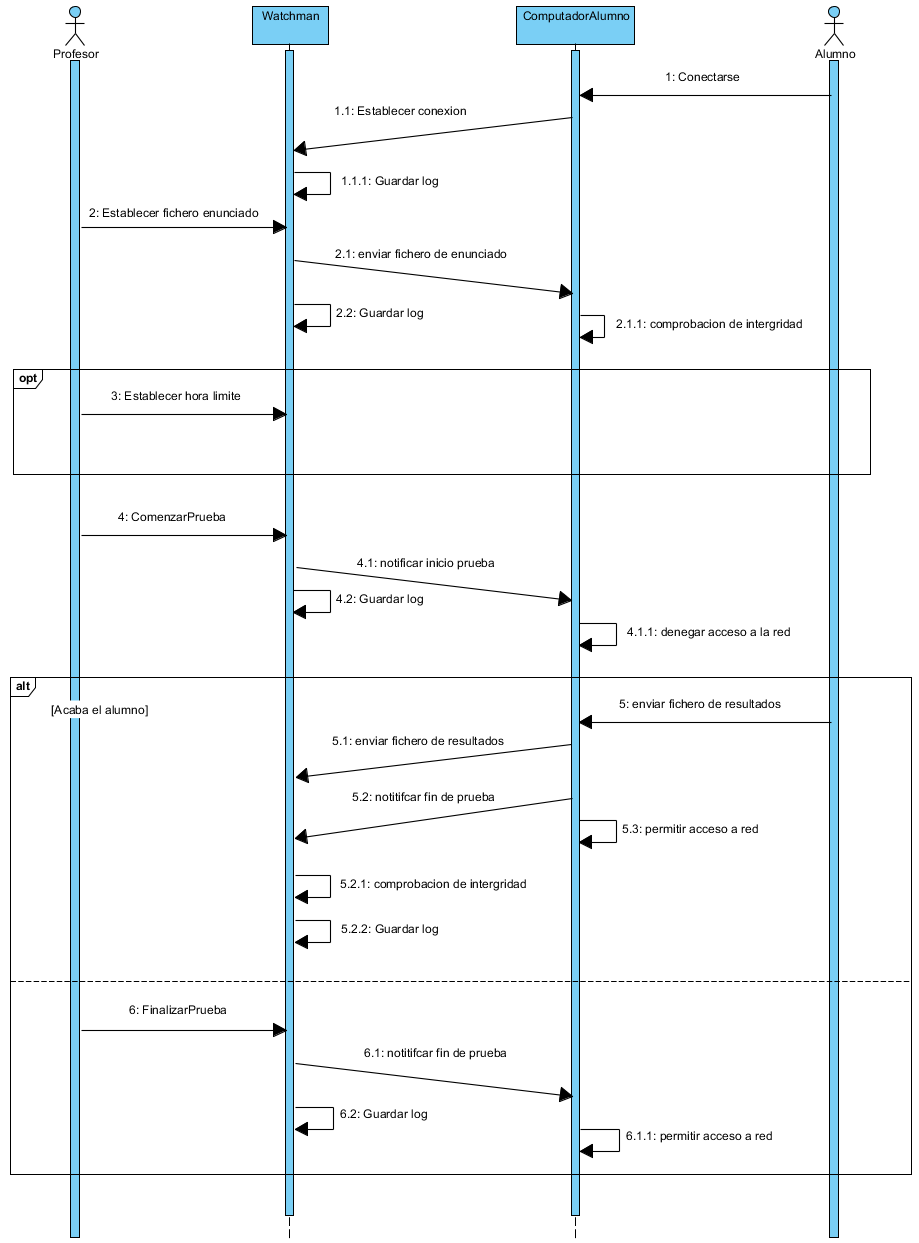
\includegraphics[width=\linewidth]{arquitectura/actividadSistema}
    \caption{Diagrama de actividad del sistema}
    \label{fig:arquitectura:actividadSistema}
\end{figure}

\section{Diseño Software}
\label{sec:arquitectura:diseno}

En esta sección se muestra en la figura \ref{fig:arquitectura:estadosAlumno} un diagrama de estados para clarificar la aplicación del alumno.
\newline


\begin{figure}
    \centering
    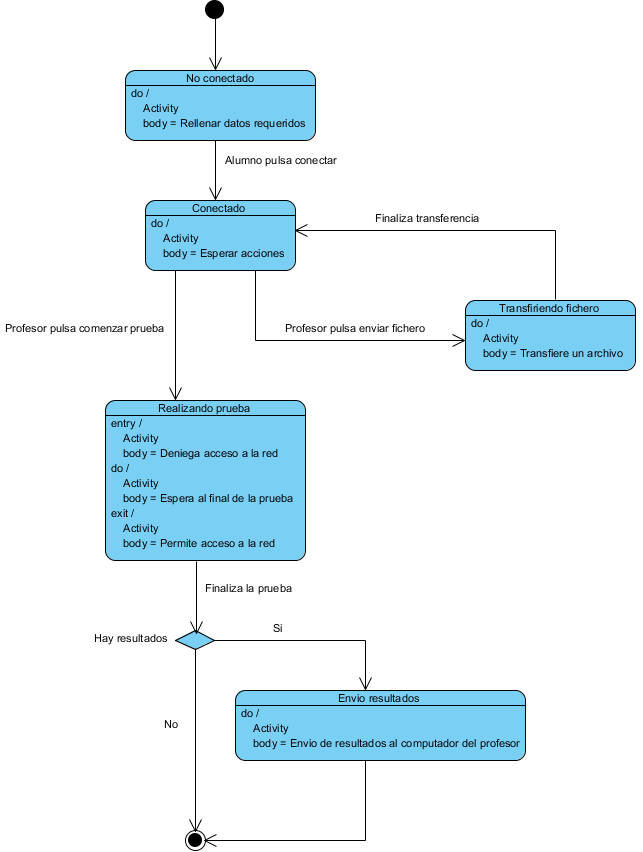
\includegraphics[width=\linewidth]{arquitectura/estadosAlumno}
    \caption{Diagrama de estados de la aplicación del alumno}
    \label{fig:arquitectura:estadosAlumno}
\end{figure}


Esa figura representa el protocolo a implementar que ha de garantizar la principal funcionalidad de la aplicación, denegar el acceso a la red en los computadores de los alumnos que están realizando la prueba, mientras esta esté en marcha, sin necesidad de apagar el router o switch del laboratorio.
\newline



El acto desactivar la red se consigue por medio de iptables, sección \ref{sec:introduction:iptables}, cambiando la política de los paquetes salientes una vez que empieza la prueba y hasta que acaba.
\newline

Por defecto iptables permite todo el tráfico que entre y salga del equipo, modificando las reglas para que deseche cualquier paquete destinado a cualquier equipo, conseguimos que no se pueda realizar ninguna petición a ningún nodo de la red, y, por tanto, tampoco recibiremos el contenido de la posible respuesta, el equipo del alumno queda aislado del resto.
\newline

A la hora de volver a permitir el acceso a la red, basta con modificar la política para el tratamiento de los paquetes salientes y restaurarla al estado anterior. Un alumno corriente no puede realizar esta operación ya que son necesarios privilegios de administrador para ello, por tanto, una vez que la aplicación desactiva la red, un alumno no puede interactuar con iptables para activarla de nuevo.
\newline


Vemos en la imagen que el único modo de finalizar la prueba es partiendo de una prueba ya iniciada, lógicamente, es decir, desde el estado \lq\lq Realizando prueba\rq\rq. Nada más entrar en este estado se desactiva el acceso a la red, por tanto, si se pretende finalizar la prueba, se ha tenido que realizar la misma sin acceso a la red. Además el acto de enviar los resultados se implementa de modo que no se pueda modificar el fichero una vez habilitada la red pero antes de transferirlo definitivamente.
\newline

Para entrar en el estado \lq\lq Realizando prueba\rq\rq, se pueden seguir dos caminos. El normal implica conectar la aplicación del alumno con la aplicación del profesor, cosa que únicamente se puede hacer antes de que dé comienzo la prueba, por tanto, tampoco se puede realizar la prueba con acceso a la red y al finalizarla, conectarse y enviar los resultados, la aplicación no aceptaría la conexión.
\newline

El otro camino involucra a una funcionalidad que tiene el sistema que consiste en permitir reconexiones de alumnos que estuviesen realizando la prueba y por el motivo que sea, un error en el sistema, por ejemplo, hayan tenido que reiniciar el computador, cuándo la aplicación del alumno vuelva a ejecutarse, al inicio de la sesión automáticamente, se reconectará con la aplicación del profesor. En la imagen se observa que sólo se puede reconectar si previamente se estaba realizando la prueba y al reconectar volveríamos automáticamente a ese estado, en el que la red se desactiva al entrar, es decir, que aunque se reinicie el computador del alumno durante el transcurso de la prueba no se conseguiría acceso a la red.
\newline




%Otro punto importante es el de la recogida de resultados automática, se ha de garantizar que el archivo no se ha corrompido a lo largo de la transferencia, para ello se realizan, tanto en el equipo que envía el fichero como en el que lo recibe, firmas MD5 al mismo para comprobar que no ha habido errores en la transferencia.


